\subsection{OCR}

OCR converts page appearance into content that other components can search or manipulate. The practical design space is broader than recognizing a string: a system may return words with coordinates, a serialized table, a structured page or a direct answer. Figure~\ref{fig:ocr_evolution} contrasts the information exposed by these interfaces.

\begin{figure*}[tp]
\centering
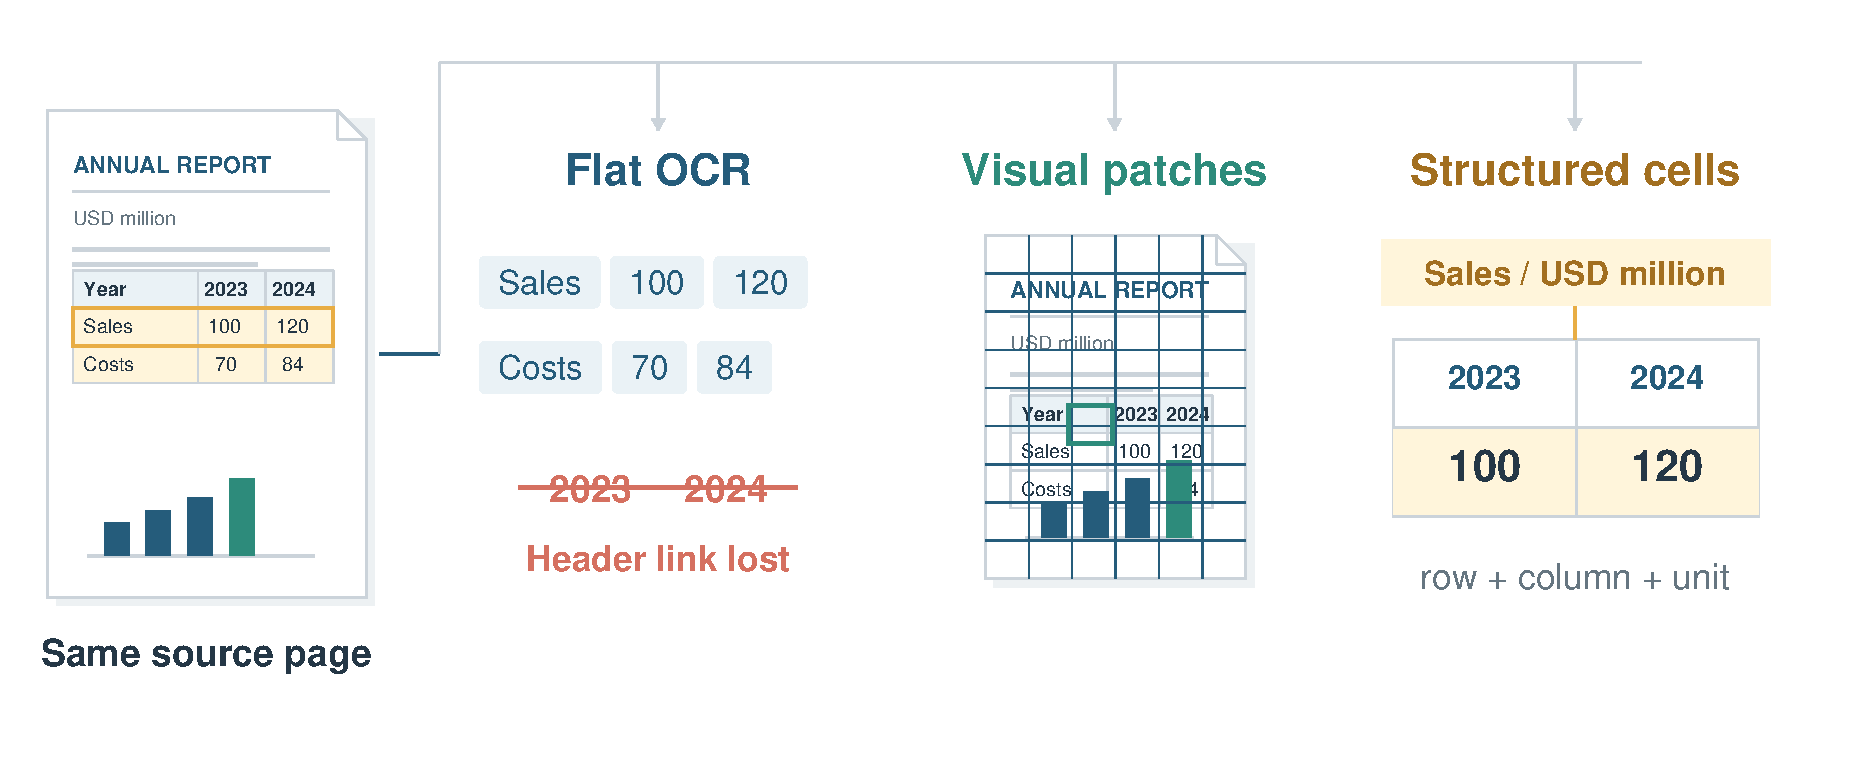
\includegraphics[width=\textwidth]{figs_by_qixingyu/fig02.pdf}
\caption{Three representations of the same page: flat OCR, visual patches and structured cells. The constructed OCR failure loses the association between values and year headers; the other panels show information that can be retained.}
\label{fig:ocr_evolution}
\end{figure*}

\subsubsection{Detection and Sequence Recognition}

A modular OCR pipeline separates page segmentation, text localization and recognition. OCRopus illustrates the combination of layout processing with learned recognition~\cite{ocropus2008}; Calamari uses convolutional and recurrent sequence modeling with CTC training~\cite{wick2018calamari}. CTC allows training from line transcripts without requiring a character boundary for every symbol, while detection supplies the regions on which recognition operates.

This separation makes errors inspectable. A missed line is a detection error; a substituted digit is a recognition error; a correct word placed in the wrong table cell is a structural assignment error. Repairing one does not automatically repair the others. Returning coordinates and page identifiers with each transcript keeps these distinctions visible to later stages.

Deployment also changes the design objective. PP-OCR optimizes a compact detection-and-recognition system~\cite{du2020ppocr}, while PaddleOCR 3.0 packages recognition, document parsing and information extraction into a broader toolkit~\cite{du2025paddleocr3}. A small recognizer may be sufficient for clean printed forms, whereas degraded scans or mixed formulas and tables can require different preprocessing and region-specific models. Architecture labels alone do not determine that trade-off.

\subsubsection{Image-to-Sequence and Vision-Language Parsing}

Generative document models decode visual features into task outputs. Donut uses an image-to-sequence interface without an external OCR transcript at inference~\cite{kim2022donut}. VISTA-OCR uses a lightweight CNN encoder and an mBART-based Transformer decoder, initialized from Donut, to autoregressively emit text and quantized coordinates~\cite{vista_ocr_2024}. Prompted transcription and localization are therefore changes to the output interface, rather than evidence that localization is unnecessary.

Vision-language OCR couples image encoding to a language model. Ocean-OCR combines a dynamic-resolution NaViT-style encoder, an MLP projector and Qwen2.5-3B~\cite{ocean_ocr_2024}. GOT addresses several content types through a unified OCR model~\cite{got_ocr_2024}; dots.ocr jointly targets layout, recognition and relations~\cite{wang2025dotsocr}. These systems can serialize heterogeneous pages, but the resulting text must still retain the distinction between a heading, a table cell and a formula.

Visual-token allocation is a central constraint. Higher resolution exposes small characters but increases the amount of visual content to encode. DeepSeek-OCR studies optical context compression~\cite{deepseek2025ocr}; TextHawk2 addresses fine-grained perception and grounding with compressed visual representations~\cite{zhang2024texthawk2}. Compression should be evaluated against the information needed by the task: a page summary may tolerate details that numerical QA cannot lose.

``OCR-free'' refers here to the absence of an external transcript at the task interface. It does not mean that the model avoids learning to read, that OCR was absent from data construction or that generated answers are grounded automatically. In the original MMLongBench-Doc experiments, most tested LVLMs underperformed the corresponding OCR-text-based LLM setting~\cite{mmlongbenchdoc2024}. That result is tied to the tested models and access conditions; it supports comparing input routes explicitly rather than treating direct visual input as a universal successor.

\subsubsection{Hybrid Parsing and Targeted Re-observation}

Hybrid systems allocate different parts of a page to different components. MonkeyOCR organizes parsing around structure, recognition and relations~\cite{li2025monkeyocr}; OCR-R1 interleaves a VLM's observations with specialist OCR tools~\cite{li2025dianjin}. A difficult formula can therefore receive different treatment from a clean paragraph. The price is an additional coordination problem: outputs from several components must agree on regions, reading order and the source of each extracted value.

The interface matters as much as the component list. A pipeline that keeps text, crops and coordinates can revisit an ambiguous digit; one that retains only plain text cannot. Conflicting tool outputs should remain associated with their source region so that a later check can compare them with the page. Calling more tools is useful only when the new observation can resolve a specific uncertainty.

OCR features can also support a task other than transcription. DocParseNet fuses visual features with OCR-derived text embeddings for semantic annotation of scanned agreements~\cite{liu2023docparsenet}. Its output identifies document regions and fields. This differs from reading every character or recovering a table's cell structure, so segmentation results should not be presented as recognition accuracy.

Table~\ref{tab:perception_routes} summarizes the resulting choices. For the financial example in Figure~\ref{fig:cross_page_case}, all routes must recover both the table and the restatement note. OCR provides inspectable strings and cells; direct visual input preserves appearance; a hybrid route can combine the two. Their shared requirement is the correct table--footnote link, not a particular model family.

\begin{table*}[tp]
\centering
\small
\setlength{\tabcolsep}{4pt}
\renewcommand{\arraystretch}{1.15}
\begin{tabularx}{\textwidth}{@{}p{0.19\textwidth}XXX@{}}
\toprule
Route & Evidence passed forward & Useful control & Main failure point \\
\midrule
Modular OCR & Text, boxes, region labels & Inspect or replace each stage & Missed text; wrong reading order \\
Text + layout & Tokens and geometry & Model spatial relations & OCR and coordinate errors \\
Direct visual & Page or crop embeddings & Retain visual appearance & Fine detail lost in resizing or compression \\
Hybrid / tools & Text, crops and linked outputs & Re-observe difficult regions & Misaligned or conflicting outputs \\
\bottomrule
\end{tabularx}
\caption{Perception routes compared by their evidence interface. These are design trade-offs, not a ranking of benchmark scores.}
\label{tab:perception_routes}
\end{table*}

\subsubsection{Evaluate the Output That the Task Uses}

Transcription, parsing and answering require different diagnostics. Character or word error measures reading fidelity, but does not test whether a table cell is attached to the right header. Parsing benchmarks inspect page structure and heterogeneous elements; answer metrics inspect the downstream result. A system may improve one while leaving another unchanged.

OCRBench aggregates 29 datasets spanning recognition and several text-dependent visual tasks~\cite{ocrbench2023}. OCRBench v2 places greater emphasis on localization and reasoning~\cite{ocrbenchv2_2024}, while OmniDocBench provides detailed annotations for diverse PDF parsing~\cite{omnidocbench2024}. Their scores answer different questions and should be reported with input resolution, page access and output requirements.

For document QA, the most useful error analysis follows a value back to its source: was the character read correctly, assigned to the right region, connected to the right label and used in the intended calculation? This separates a recognizer improvement from a structural or reasoning improvement. It also identifies when another crop or a specialist tool is warranted, instead of escalating every page to a more complex pipeline.
